\documentclass{article}

\usepackage[italian]{babel}
\usepackage[utf8]{inputenc}
\usepackage{graphicx}

\author{Fabio Biselli}
\title{Progetto: modello astratto}
\date{}

\begin{document}

\maketitle

\section{Il sistema in sintesi}
Il sistema introdotto nell'articolo ed illustrato in figura \ref{fig1}
è così composto:
\begin{itemize}
\item
3 server, di cui uno contrassegnato come principale;
\item
180 client che controllano un avatar nel mondo virtuale;
\item
Una rete che connette i client ai server (che sono tra loro interconnessi);
\item
Un'area di gioco (Virtual Environment);
\item
Un metodo ed un file di partizionamento che il server principale utilizza per
suddividere il carico tra i server.
\end{itemize}

Il sistema di partizionamento per l'assegnamento dei client ad un server è
basato sul concetto di Area d'Interesse di un avatar (AoI). Ovvero se due
avatar condividono la medesima AoI dovrebbero essere gestiti dal medesimo
server.

All'inizio della simulazione gli avatar (client) sono distribuiti nel'area
di gioco in modo uniforme.  

La simulazione consiste nel far compiere ad ogni avatar 100 movimenti, uno
ogni 2 secondi. Quando l'avatar compie un movimento invia un messaggio di
ACK al server associato che lo propaga ai client nella relativa AoI.
I client che ricevono l'ACK rispediscono il messaggio al server che notifica
l'ACK ricevuto al client che ha effettuato lo spostamento. In questo modo è
possibile calcolare i tempi di risposta del sistema.
Alla fine della simulazione ogni client può calcolare il tempo medio di
risposta del sistema.

\begin{figure}
\label{fig1}
\begin{center}
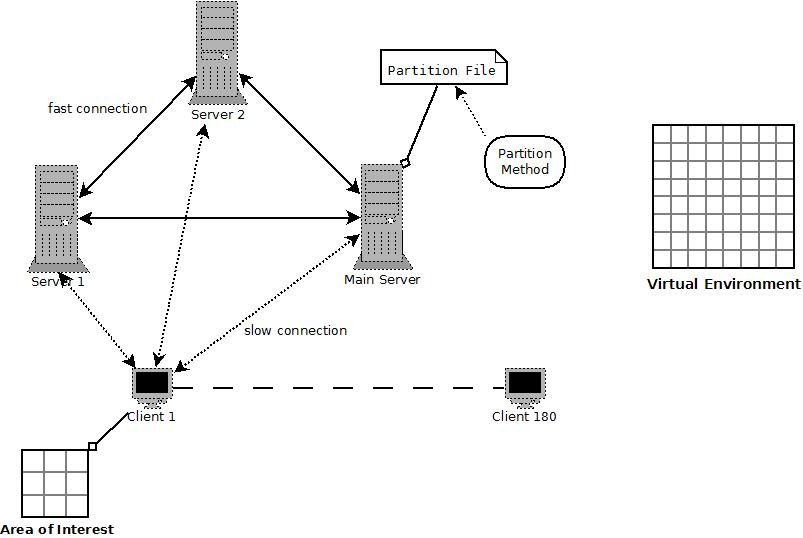
\includegraphics[scale=0.50]{schema.jpeg}
\end{center}
\caption{Schema proposto nell'articolo di riferimento.}
\end{figure}

\section{Alcune idee per l'implementazione}

Per quanto riguarda l'implementazione del modello di cui sopra seguono le
principali caratteristiche da implementare.

\subsection{Impostazioni iniziali}
Nell'articolo vengono descritte due diverse simulazioni con numeri di server
e client fissi. L'implementazione di questa simulazione, basata su OMNet++,
prevede un numero parametrico di server e client in modo tale che l'utente
possa specificarne il numero. 

Si suppone che inizialmente gli avatar siano distribuiti nel mondo con una
data distribuzione.

\subsection{Area di gioco}
L'area di gioco è una semplicissima struttura: un array
bidimensionale di puntatori ad una lista di Avatar (AvatarList). Questa
"simula" un'area di gioco in cui gli avatar possono muoversi liberamente e
senza collisioni.

\subsection{Avatar}
Avatar è una semplice classe che rappresenta un client. Ha due campi:
un indice che si riferisce al client (getIndex() in simpleModule di OMNet) ed
una lista di indici che rappresentano gli altri avatar nella propria AoI.

\subsection{Gestione area di gioco e movimenti}
L'area di gioco viene modificata dai server che, grazie alle notifiche dei
movimenti da parte dei client, rimuovono l'avatar dal vecchio puntatore
(o lista) e lo assegnano a quello di destinazione. Quindi vengono aggiornati
gli avatar coinvolti, ovvero quando un avatar si sposta il server:
\begin{enumerate}
\item
notifica ai vicini che l'avatar lascia la casella;
\item
calcola una nuova AoI con i nuovi vicini;
\item
notifica ai nuovi vicini l'ingresso dell'avatar nella casella di
destinazione.
\end{enumerate}

I movimenti degli avatar, che avverranno ogni due secondi, avranno come
destinazione una delle caselle adiacenti (compresa la casella di partenza,
in tal caso nessun messaggio sarà inoltrato nel sistema). Tuttavia, con una
piccola probabilità, ogni avatar potrà effettuare un "Jump" ad una casella
casuale nel mondo, come evento eccezionale.

\subsection{Connessioni}
I server sono interconnessi, mediante dei "channel" con un basso delay
per simulare una connessione intranet (LAN) fra loro. Mentre per le connessioni
Client-Server i canali hanno una latenza più alta e variabile per 
simulare una WAN.

\subsection{Metodo di partizionamento}
Il metodo di partizionamento, poiché non è oggetto dello studio, sarà
implementato in modo semplificato. Ad ogni Server sarà assegnata una porzione
del mondo in modo lineare. Questo introdurrà un numero massimo di server che
l'utente potrà specificare all'avvio.

\begin{figure}
\label{fig2}
\begin{center}
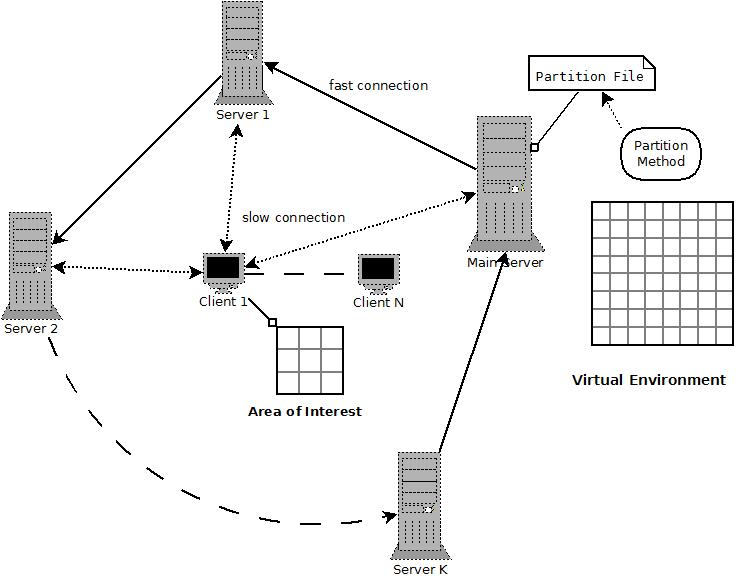
\includegraphics[scale=0.50]{schemaRing.jpeg}
\end{center}
\caption{Schema proposto per l'implementazione.}
\end{figure}

\end{document}